\subsection{Parametrische Darstellung}
Die Übergangsfunktion $h(t)$ erhält man, indem man die Laplace-Rücktransformierte der Übertragungsfunktion bildet. In Matlab lässt sich das durch folgende Befehle bewerkstelligen:\\
\hspace*{0.5cm}\texttt{syms s t}\\
\hspace*{0.5cm}\texttt{G(s) = -25/(10*s+1)}\\
\hspace*{0.5cm}\texttt{h(t) = ilaplace(G(s)/s)}\\
Alternativ lässt sich die Übertragungsfunktion auch durch Integration der Gewichtsfunktion berechnen. In Matlab benötigt man dafür folgende Befehle:\\
\hspace*{0.5cm}\texttt{g(t) = ilaplace(G(s))}\\
\hspace*{0.5cm}\texttt{h(t) = int(g(t), 0, t)}\\
Beide Berechnungen liefern uns das Ergebnis:
\begin{equation*}
    h(t) = 25*e^{\frac{-t}{10}}-25
\end{equation*}

% Hier graphisch dargestellt:
% \begin{figure}[H]
%     \centering
%     \includegraphics[width=8cm]{image/Übergangsfunktion.eps}
%     \caption{Übergangsfunktion $h(t)$}
% \end{figure}


\subsection{Nichtparametrische Darstellung}
\subsubsection{Plot mit Matlab}
Nach der Berechnung der Übergangsfunktion lässt sich diese durch folgende Befehle in Matlab plotten:\\
\texttt{t=[0:10:100]}\\
\texttt{plot(t, (25)*exp(-t/10)-25)}\\
Durch diese Befehle liefert Matlab folgendes Ergebnis (siehe Abbildung 1):
\begin{figure}[H]
    \centering
    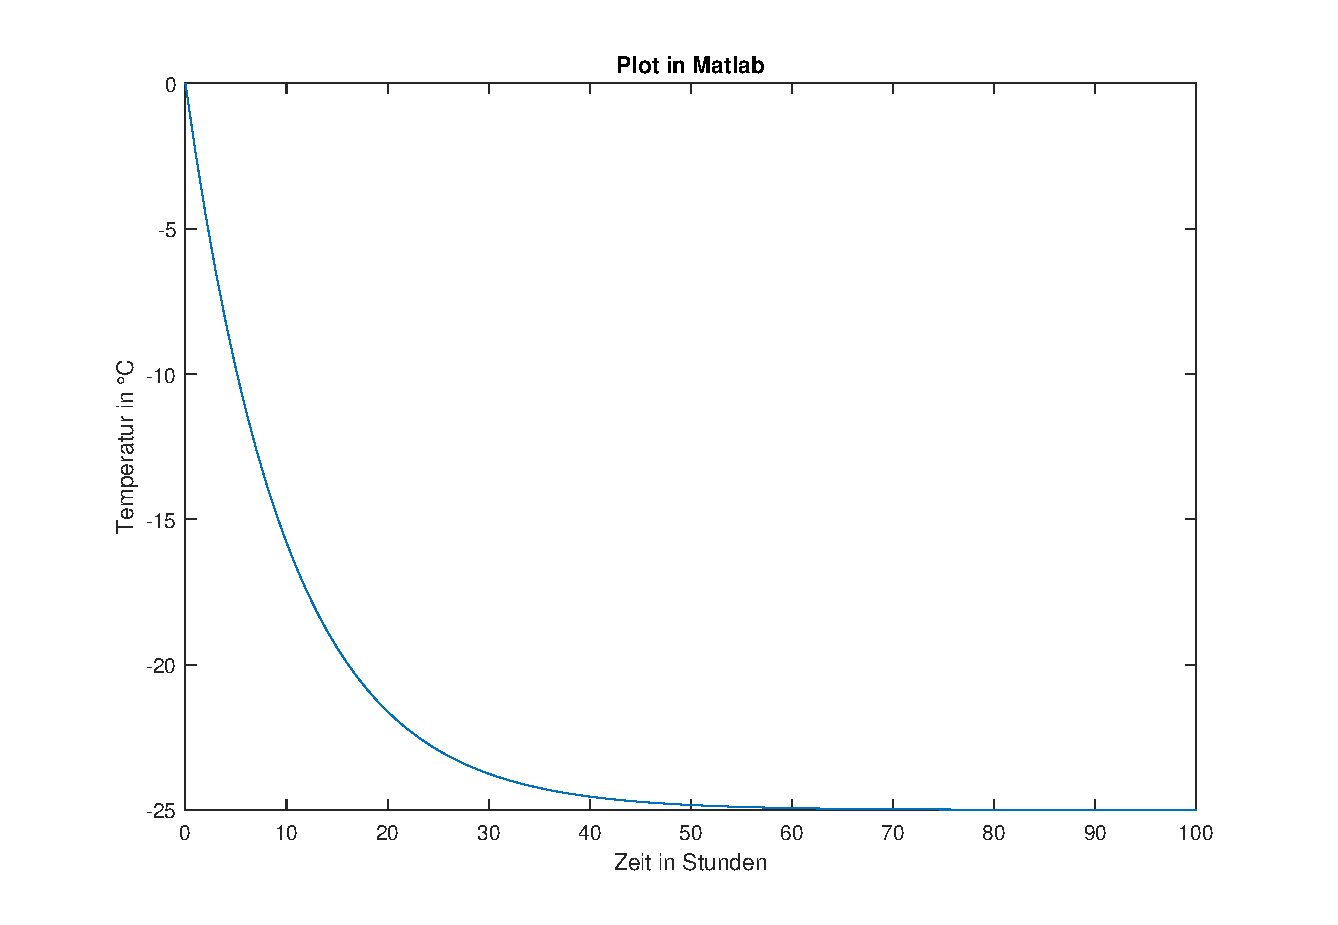
\includegraphics[width=12cm]{images_2/Übergangsfunktion/Übergangsfkt_plot_matlab.eps}
    \caption{Sprungantwort: Plot mit Matlab}
\end{figure}

\subsubsection{Plot mit Step-Funktion}
Den selben Plot erhält man in Matlab auch über die \texttt{step}-Funktion. Diese lässt sich durch folgende Befehle anzeigen:\\
\hspace*{0.5cm}\texttt{sys = tf([-25],[10 1])}\\
\hspace*{0.5cm}\texttt{step(sys)}\\
Das von Matlab gelieferte Ergebnis ist in Abbildung 2 dargestellt.
\begin{figure}[H]
    \centering
    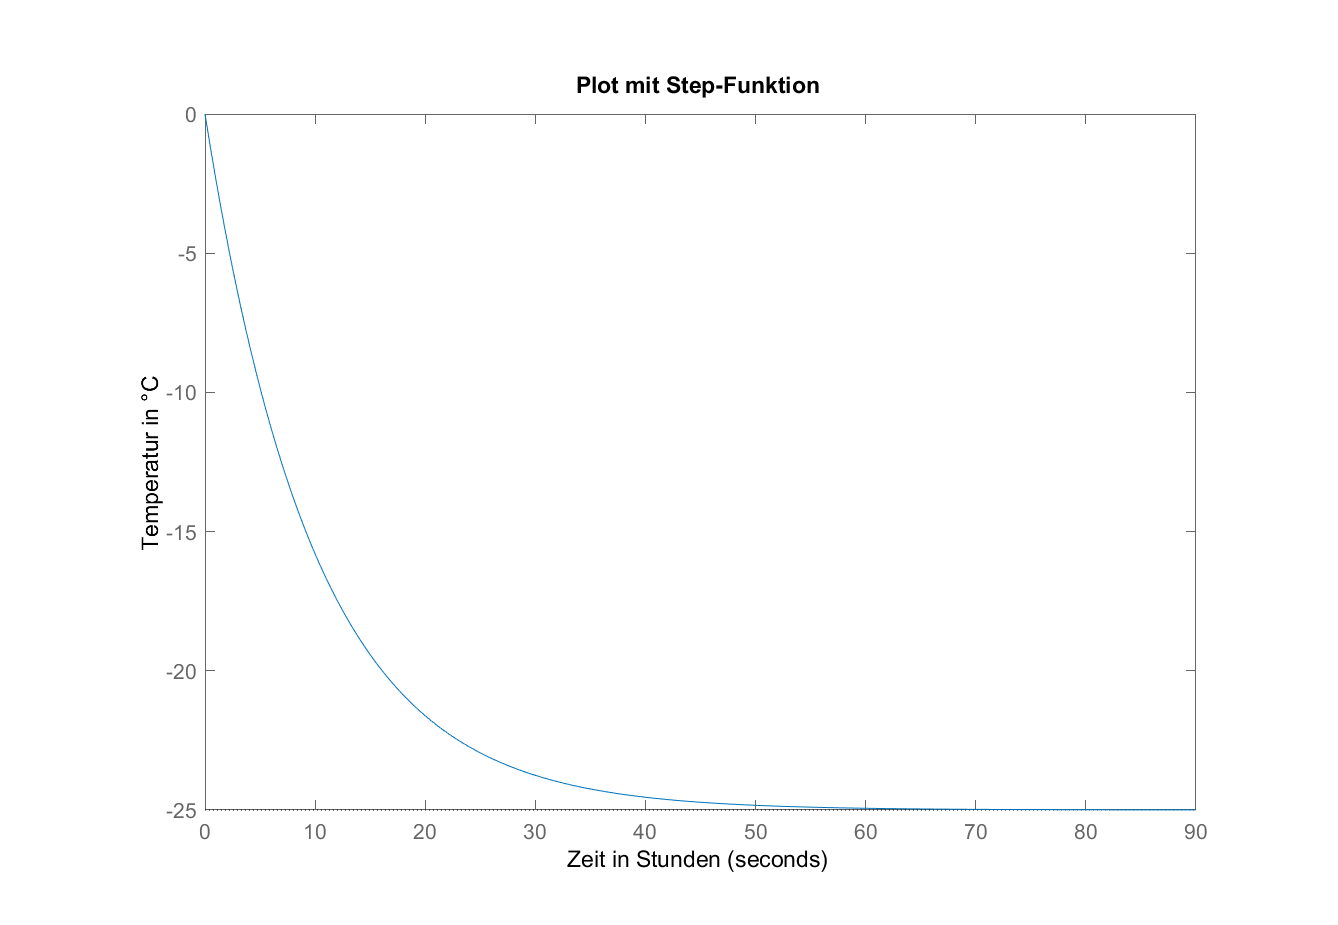
\includegraphics[width=12cm]{images_2/Übergangsfunktion/Übergangsfkt_plot_stepfunktion.eps}
    \caption{Sprungantwort: Plot mit Step-Funktion}
\end{figure}

\subsubsection{Plot mit Simulink}
Das selbe Ergebnis lässt sich ebenfalls in Simulink durch folgende Schaltung erzielen:
\begin{figure}[H]
    \centering
    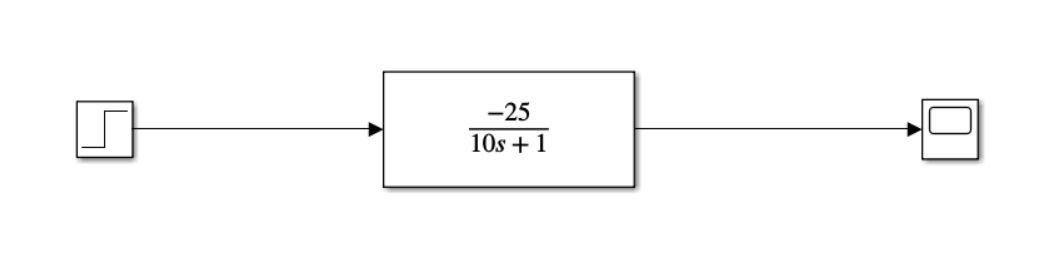
\includegraphics[width=13cm]{images_2/Übergangsfunktion/simulink-schaltung.png}
    \caption{Sprungantwort: Simulink Schaltung}
\end{figure}
\begin{figure}[H]
    \centering
    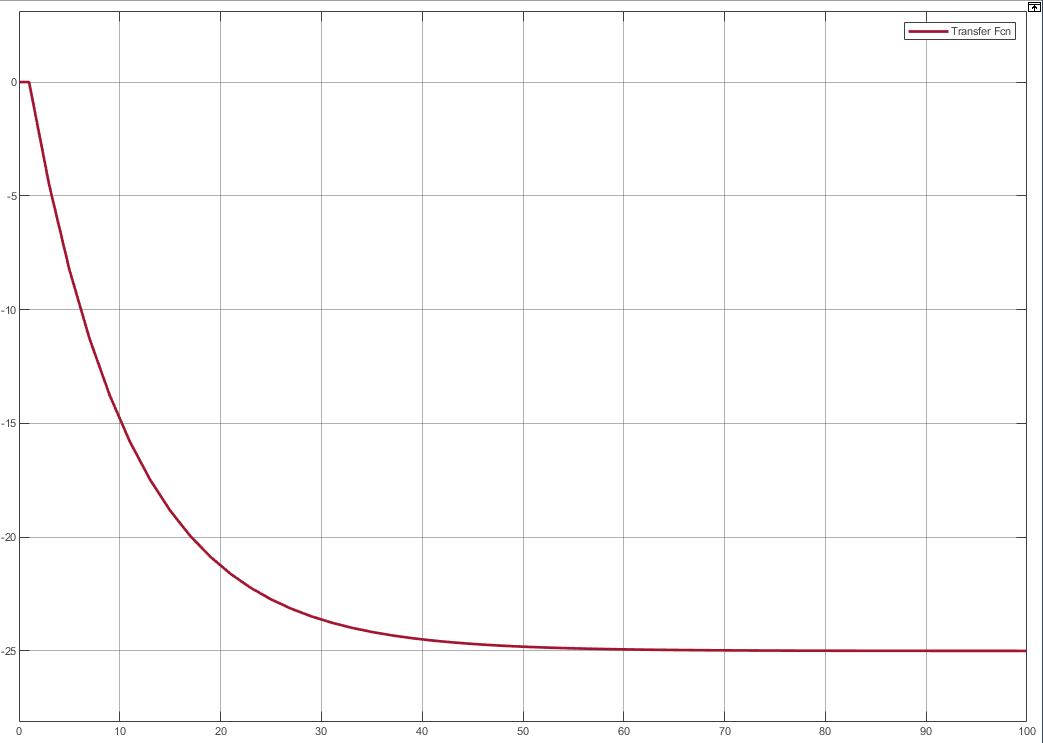
\includegraphics[width=10cm]{images_2/Übergangsfunktion/übergangsfkt_simulink-plot.png}
    \caption{Sprungantwort: Plot mit Simulink}
\end{figure}












% Da t ein Vektor ist, muss man beim Multiplizieren das Punktprodukt (Hadammad-Produkt) verwenden.

        
%Die Control System Toolbox dient der systematischen Analyse, dem Entwurf und der Optimierung linearer Systeme.\\
%Mit dem folgenden Matlab-Skript kann ich die Übertragungsfunktion G(s) in MATLAB eingeben.
%\lstinputlisting[style=Matlab-editor, caption={pretty}]{../MATLAB/ControlSystemToolbox/cst_DTs.m}
%Lässt man sich G(s) in der Konsole anzeigen, wird diese folgendermaßen dargestellt.
                    
%Durch den Befehl \texttt{step(sys)} öffnet MATLAB ein neues Fenster mit der passenden Sprungantwort h(s) zu G(s) und stellt diese folgendermaßen dar.



